\documentclass[a4paper,12pt]{article}
\usepackage{amsfonts,amssymb}
\usepackage{graphicx}
\usepackage{algorithm,algorithmic}
\usepackage{multicol}
\usepackage{multirow}
\usepackage{etoc}
\usepackage{subcaption}
\title{User Manual}
\author{}
\date{}
\begin{document}
	\maketitle
	\tableofcontents
	\etocsettocstyle{\subsection*{This Chapter contains:}}{\noindent\rule{\linewidth}{.4pt}}
	


\section{Introduction}
This document describes how to use \emph{Triangle Algorithm} and \emph{Spherical Triangle Algorithm}, which are part of a Matlab package for \textit{Convex Hull Membership } (CHM) problems, a fundamental problem in Linear Programming, Computational Geometry, Machine Learning and Statistics. It also serves as a query problem in many applications, e.g., Topic Modeling, LP Feasibility and Data Reduction. Definitions and technical details are included in the main article \cite{kalantari20191}.


\section{Installation}
The algorithms are implemented using Matlab 2019 \footnote{Any advice or opinions posted here are our own, and in no way reflect that of MathWorks.}. To begin, one needs to install Matlab. The algorithms also works on Octave 5.2.0 with additional statistics package.  Having started Matlab, access to all the user callable functions is obtained using:
\begin{verbatim}
%%%
addpath(Directory containing Spherical Triangle Algorithm)
%%%
\end{verbatim}
Note that the path needs to be added each time Matlab is started.
\section{Main Functions}


\subsection{$Tri\_algo$}
\begin{verbatim}
[inorout,p_prime,alpha_coe,gap,iter_num]...
=Tri_Algo(input_a,epsilon,query,varargin)
\end{verbatim}
\subsubsection*{Description}
	The function \texttt{Tri\_algo} is an implementation of the {\it Triangle Algorithm} (TA)  described in \cite{kalantari2015characterization}. The Triangle Algorithm is an iterative algorithm for solving the approximate CHM problem : given a set $S=\{v_1, \dots, v_n\} \subset \mathbb{R}^m$, a distinguished point $p \in \mathbb{R} ^m$, and $\varepsilon \in (0,1)$, solving CHM means either computing an $\varepsilon$-{\it approximate solution}, i.e. $p_\varepsilon \in conv(S)$ so that  $\Vert p - p_\varepsilon \Vert  \leq \varepsilon R,  \quad R = \max \{\Vert v_i - p \Vert  : v_i \in S\}$ 	or {\it witness}: a point $p' \in conv(S)$ for which  there is no $v \in S$ with  $\Vert p' - v \Vert \geq \Vert p - v \Vert$. If $p'$ is a witness,
	the orthogonal bisecting hyperplane to $pp'$ separates $p$ from $conv(S)$. 

\subsubsection*{Parameters}


\noindent Input:
\begin{itemize}
	\item {$input\_a$:}
	An $m \times n$ dimensional matrix representing the set of $n$ points in dimension $m$.

	\item {$epsilon$:}
	A scalar in $(0,1)$; precision parameter. In practice, the $epsilon$ is usually chosen between $[0.01,0.001]$. The number of iteration in the worst case has $O(1/\varepsilon^2)$ iterations.
 	\item {$varargin$:}
	This variable is set to be an  $n\times 1$ vector with non-negative entries that sum up to $1$ if manual initialization is used.  Otherwise leave it blank.
	\item {$query$:}
	An $m\times 1$ vector representing $p$, the query point in dimension $m$.
\end{itemize}
Output:
\begin{itemize}
	\item {$innout$:}
	${0,1}$ binary scalar. Its value is $0$ if a witness is found, $1$ if an $\epsilon$-approximation solution is found.  
	\item {$alpha\_coe$ :}
	An $n\times 1$ vector. The value of $\alpha$ so that $A\alpha=p'$ where $p'$ is an $\varepsilon$ solution.
	\item {$p\_prime$:}
	An $m\times1$ vector. Witness or an $\varepsilon$-approximation solution  of query point.
	\item {$gap$:}
	Euclidean distance between $p\_prime$ and query point $p$.
	\item {$iter\_num$:}
	Number of iterations for algorithm to stop.
\end{itemize}





\subsubsection*{Examples}
This example uses  \texttt{Tri\_algo} to solve the convex hull membership problem. For simplicity, the data points are generated from a unit sphere. The query point  $p$ is generated using a random convex combination of the given set of points. In the example the number of points, $n$, is set to 20 and the dimension, $m$, to 10.
\begin{verbatim}
m=10;
n=20;
epsilon=0.01;
%% Generate points from unit sphere
matA=Random_pts(m,n,'unit ball'); 
%%
%% query points p is in the convex hull
p=Random_cvx(matA,1);
%%
tic
[inorout,p_prime,alpha_coe,gap,iter_num]...
=Tri_Algo(matA,epsilon,p);
toc
alpha_coe
p_prime 
inorout
dist
\end{verbatim}
The output of above program is:\\
\begin{multicols}{1}
	\begin{verbatim}
	alpha_coe
	=
	      0
	0.0137
	0.0355
	0.0239
	0.2518
	0.1666
	0.0676
	0
	0
	0
	0
	0.0495
	0.2012
	0
	0
	0.0616
	0.0122
	0
	0.0417
	0.0745
	\end{verbatim}
	\columnbreak
	\begin{verbatim}
	p_prime 
	=
	0.0008
	-0.0611
	-0.0220
	-0.0541
	0.0501
	-0.0826
	-0.0605
	-0.0270
	0.0398
	0.0310
	\end{verbatim}
	\columnbreak
\end{multicols}	
	\begin{verbatim}
inorout =1
dist=0.0104
Elapsed time is 
0.032385 seconds.
\end{verbatim}


%\subsection{Main Function}
\subsection{$Spherical\_TA$}
\begin{verbatim}
[innout,p_prime,alpha_coe,gap,iter_num]...
=Spherical_TA(input_a,epsilon,alpha_0,query)
\end{verbatim}
\subsubsection*{Description}
\texttt{Spherical\_TA} is an implementation of the {\it Spherical Triangle Algorithm}, which solves the CHM problem by converting a CHM into a spherical CHM.  The {\it Spherical-CHM} is the case of CHM, where $p=0$ and each $v_i \in S$ has unit norm.  Given a data set $S^r=\{v_1^r,...v^r_n\}$ and $p^r$, we set $p=0$ and set $S=\{v_1,...,v_n\}$, where $v_i=(v^r_i-p^r)/\|v^r_i-p^r\|$. This step scales every point onto a unit sphere. The function \texttt{Spherical\_TA} then applies the Triangle Algorithm to solve the scaled problem. The solution to the Spherical CHM is then converted back to a solution of the original CHM query. Details are provided in ~\cite{kalantari20191}.

%\begin{algorithm}[H]
%	\caption{Spherical-TA ($S^r=\{v_1^r,...,v^r_n\}$, $p^r$, $\varepsilon \in (0,1)$)}
%	\begin{algorithmic}[1]
%		\scriptsize
%		\STATE	{\bf Step 0.} Compute $S=\{v_1,...,v_n\}$ where $v_i=(v^r_i-p^r)/\|v^r_i-p^r\|$. Set $p=0$.
%		%Scale all $v_i$ on to unit sphere. Set $p=0$.
%		\STATE 	{\bf Step 1.}  Set $p'= v_1$.
%		\STATE  {\bf Step 2.} If $\Vert p'\Vert \leq \varepsilon$, then output $p'$ as an $\varepsilon$-approximate solution, stop.
%		\STATE 	{\bf Step 3.}  If there is a strict pivot $v_j \in S$, set $p' \leftarrow Nearest(0; p'v_j )$. Goto Step 1.
%		\STATE 	{\bf Step 4.} Output $p'$ as a witness. Stop.	
%	\end{algorithmic}
%\end{algorithm}

\subsubsection*{Implementation}

\noindent Input:
\begin{itemize}
	\item {$input\_a$:}
	 An $m \times n$ dimensional matrix representing the set of $n$ points in dimension $m$.
	\item {$epsilon$:}
	A scalar in $(0,1)$; precision parameter. In practice, the $epsilon$ is usually chosen between $[0.01,0.001]$. The number of iteration in the worst case has $O(1/\varepsilon^2)$ iterations.
	\item {$alpha\_0$:}
	 An $n\times 1$ vector with non negative entries that sum up to $1$; initialization of the coefficient.
	\item {$query$:}
	 An $m\times 1$ vector representing the query point $p$ in dimension $m$.
\end{itemize}
Output:
\begin{itemize}
	\item {$innout$:}
${0,1}$ binary scalar. Its value is $0$ if a witness is found, and $1$ if an $\epsilon$ approximation solution is found.  
\item {$alpha_coe$ :}
An $n\times 1$ vector. The value of $\alpha$ so that $A\alpha=p'$ where $p'$ is an $\varepsilon$ solution.
\item {$p\_prime$:}
An $m\times1$ vector. Witness or an $\varepsilon$-approximation solution of query point.
\item {$gap$:}
Euclidean distance between $p\_prime$ and the query point $p$.
\item {$iter\_num$:}
Number of iterations for the  algorithm to stop.
\end{itemize}

\subsubsection*{Examples}

This example uses \texttt{Spherical\_TA} to solve CHM.  For simplicity, the data points are generated from a unit sphere. The query point  $p$ is generated using a random convex combination of a given set of points. In the example the number of points, $n$, is set to 20 and the dimension, $m$, to 10.
\begin{verbatim}
	m=10;
	n=20;
	%% Generate points from unit sphere
	matA=Random_pts(m,n,'unit ball'); 
	%%
	%% query points p is in the convex hull
	p=Random_cvx(matA,1);
	%%
	tic
	[inorout,p_prime,alpha_coe,gap,iter_num]...
	=Spherical_TA(matA,epsilon,zeros(n,1),p);
	toc
	alpha_coe
	p_prime 
	inorout
	dist
\end{verbatim}
The output of above program is:\\
\begin{verbatim}
alpha_coe
=
0.0482
0
0.1060
0.0288
0
0.0461
0.0057
0
0
0
0.0180
0.0243
0.0101
0.2003
0.0206
0.2211
0
0.1607
0.0279
0.0820
\end{verbatim}
\begin{verbatim}
p_prime 
=
-0.0038
0.0006
-0.0163
0.0006
-0.0048
0.0076
-0.0015
0.0036
0.0074
0.0005
\end{verbatim}
\begin{verbatim}
inorout =1
dist=0.0058
Elapsed time is 
0.019650 seconds.
\end{verbatim}

\subsection{$AVTA\_PLUS$}
\begin{verbatim}
[index]=AVTA_PLUS(matrix_A,gamma,varargin)
\end{verbatim}
\subsubsection*{Description}
The function \texttt{AVTA\_PLUS} is an implementation of $AVTA+$ in \cite{kalantari20191}. $AVTA$ \cite{pmlr-v84-awasthi18a} solves the exact or approximate version of the {\it irredundancy problem} ~\cite{toth2017handbook}: given a set of $n$ points $S=\{v_1,\dots,v_n\}$ in $\mathbb{ R}^m$, it computes all vertices of its convex hull.  $AVTA+$ replaces the use of Triangle Algorithm in AVTA by  Spherical-TA as a faster membership query oracle. The function also includes an implementation of J-L random projection \cite{johnson1984extensions} for dimension reduction.\\

\noindent Input:
\begin{itemize}
	\item {$matrix\_A$:}
	An $m \times n$ matrix representing set of $n$ points in dimension $m$.
	\item {$gamma$:}
	A scalar in $(0,1)$; precision parameter.In practice, the $gamma$ is usually chosen between $[0.05,0.001]$. 
	\item {$varargin$:}
	 If random projection is used for dimension reduction, this variable is set to be  $'Rp'$, dimension of random projection. Otherwise leave it blank. For example,\\ \texttt{[index]=AVTA\_PLUS(matrix\_A,gamma,$'Rp'$,50)} \\
	 uses random projection with dimension $50$. \\
	 \texttt{[index]=AVTA\_PLUS(matrix\_A,gamma)}\\
	 doesn't not apply random projection.
	 
\end{itemize}
Output:
\begin{itemize}
	\item {$index$:}
	Integer vector, subset of  $[n]$. Index of vertices. 
\end{itemize}


This example uses \texttt{AVTA\_PLUS} to solve the irredundancy problem using points generated from a unit sphere.The problem specified below uses $n=100$ points, dimension $m=10$ and $K=20$ vertices.
\begin{verbatim}
m=20;
K=20;
n=100;
vtx_A=Random_pts(m,K,'normal');
inhulldata=Random_cvx(vtx_A,n,'unif');
matA=[inhulldata,vtx_A];
[m,n]=size(matA);
tic
[index]=AVTA_PLUS(matA,0.01);
toc
index
\end{verbatim}
The output of above program is:\\

\begin{verbatim}
Elapsed time is 
0.181165 seconds.

index =
101
102
103
104
105
106
107
108
109
110
111
112
113
114
115
116
117
118
119
120
\end{verbatim}



\section{Auxiliary Functions}

\subsection{$Random\_pts$}

\begin{verbatim}
[mat_A]=Random_pts(m,n,varargin)
%%This function generates random data points.
\end{verbatim}

\noindent Input:
\begin{itemize}
	\item {$n$:}
	Number of points. 
	\item {$m$:}
	Dimension.
	\item {$varargin$:}
	\begin{itemize}
		\item 
		$'normal` $: The data points are generated using standard Gaussian distributution.
		\item 
		$'unif` $: Thedata points are generated using  standard uniform distribution.
		\item 
		$'unit ball`$: The data points are uniformly generated on a unit sphere.
	\end{itemize}

\end{itemize}
Output:
\begin{itemize}
	\item {$mat\_A$:}
	The $m \times n$ matrix containing the set of random generated points.
\end{itemize}

\subsection{$Random\_cvx$}
\begin{verbatim}
[mat_A]=Random_cvx(vtx_A,n,varargin)
%% Given a set of points as generators, this function generates n 
%% points using a convex combination of the generators. 
\end{verbatim}

\noindent Input:
\begin{itemize}
	\item {$n$:}
	Number of points. 
	\item {$m$:}
	Dimension.
	\item {$varargin$:}
	\begin{itemize}
		\item 
		$['dir',para]$ :  The data points are generated using the standard dirichlet distribution with $para$ as hyper parameter.
		\item 
		$'unif`$:  The data points are generated using the scaled standard uniform distribution
	\end{itemize}
\end{itemize}
Output:
\begin{itemize}
		\item {$mat\_A$:}
	The $m \times n$ matrix representing set of random generated points.
\end{itemize}

\section{Demo}

	%
\noindent The \texttt{Demo.m }driver uses data generated using a Gaussian distribution. Following three algorithms are used to solve  the CHM problem:  the Simplex method ~\cite{chvatal1983linear} (using package provided by Matlab),  the TA ~\cite{kalantari2015characterization}, and the Spherical-TA. The output in  Figure ~\ref{fig1} consists of two plots that compare the run times of the three methods on all the tests executed. The two plots corresponds to the two cases in CHM when the query $p$ is feasible or infeasible. 


\begin{verbatim}
%%%%%%%%%%%%%%%%%%%%%%%%%%%%%%%%%%%%%%%%%%%%%%%%%%%%%%%%%%
%% This is a demo for Spherical Triangle Algrithm
%% Full paper available on Arxiv:
%% Spherical Triangle Algorithm: A Fast 
%% Oracle for Convex Hull Membership Queries
%%%%%%%%%%%%%%%%%%%%%%%%%%%%%%%%%%%%%%%%%%%%%%%%%%%%%%%%%




clear all
options = optimset('linprog');
options.Display = 'off';
%% Number of repetition
Num_rep=3; 
%%
%% Problem size (dim,number of points)
Problem_size=[100,1000;200,2000;500,5000;1000,10000]; 
%%
%% Precision parameter
epsilon=0.01; 
%%

%%%%%%%%%%%%%%%%%%%%%%%%%%%%%%%%%%
%%Query point infeasible
%%%%%%%%%%%%%%%%%%%%%%%%%%%%%%%%%%
%%Triangle Algorithm running time
time_ta=zeros(1, length(Problem_size(:,1))); 
%%
%%Spherical Triangle Algorithm running time
time_sphere_ta=zeros(1, length(Problem_size(:,1))); 
%%
%% Linear Programming running time
time_lp=zeros(1, length(Problem_size(:,1)));  
%%
%% Itertion number Spherical Triangle Algorithm
iter_ta=zeros(1, length(Problem_size(:,1)));     
%%
%% Itertion number Triangle Algorithm
iter_sphere_ta=zeros(1, length(Problem_size(:,1))); 
%%
for ii=1:length(Problem_size(:,1))
Num_dim=Problem_size(ii,1);
Num_vtx=Problem_size(ii,2);
for kk=1:Num_rep
%%%Data generation
vtx_A=Random_pts(Num_dim,Num_vtx,'normal');
matA=vtx_A;
[m,n]=size(matA);
%p=Random_cvx(vtx_A,1,'dir');%% Query points
p=Random_pts(Num_dim,1,'normal');
%%%
disp('Triangle Algorithm starts')
%%Triangle Algorithm
tic;
[inorout,p_prime,alpha_coe,dist,ta_iter]=Tri_Algo(matA,epsilon,p);
ta_end=toc;
time_ta(ii)=time_ta(ii)+ta_end;
iter_ta(ii)=iter_ta(ii)+ta_iter;
disp('Triangle Algorithm time')
disp(ta_end)
%%Spherical Triangle Algorithm
disp('Spherical Triangle Algorithm  starts')
tic;
[inorout,p_prime,alpha_coe,dist,iter_num]...
=Spherical_TA(matA,epsilon,zeros(n,1),p);
sphere_ta_end=toc;
time_sphere_ta(ii)=time_sphere_ta(ii)+sphere_ta_end;
iter_sphere_ta(ii)=iter_sphere_ta(ii)+iter_num;
disp('Spherical Triangle Algorithm  time')
disp(sphere_ta_end)
%%Linear Programming
disp('Linear Programming starts')
tic;

n_var=n;
n_con=m;
x_y_size=n_con+n_var;
cvx_aeq=ones(1,n_var);
Aeq=[matA,eye(n_con);ones(1,n_var),zeros(1,n_con)];
beq=[p;1];
lb=zeros(x_y_size,1);
tic
options = optimset('linprog');
options.Display = 'off';

[bb,fval] = linprog([zeros(n_var,1);ones(n_con,1)],[],[]...
,Aeq,beq,lb,[],options);
lp_t=toc;
time_lp(ii)=time_lp(ii)+lp_t;
disp('Linear Programming time')
disp(lp_t)
end  
end

figure(1);
hold on
title('query point infeasible')
plot(log((time_ta(1,:))),'DisplayName','TA','LineWidth',1.5)
plot(log((time_sphere_ta(1,:))),'DisplayName',...
'Spherical TA','LineWidth',1.5)  
plot(log(time_lp(1,:)),'DisplayName','LP','LineWidth',1.5)  ;
% plot(mean(time_mirror_ta(2,:)))  
legend('show','Location','northwest')%,'Orientation','horizontal')
hold off;










%%%%%%%%%%%%%%%%%%%%%%%%%%%%%%%%%
%%%%Query point feasible
%%%%%%%%%%%%%%%%%%%%%%%%%%%%%%%%%



%%Triangle Algorithm running time
time_ta=zeros(1, length(Problem_size(:,1))); 
%%
%%Spherical Triangle Algorithm running time
time_sphere_ta=zeros(1, length(Problem_size(:,1))); 
%%
%% Linear Programming running time
time_lp=zeros(1, length(Problem_size(:,1)));  
%%
%% Itertion number Spherical Triangle Algorithm
iter_ta=zeros(1, length(Problem_size(:,1)));     
%%
%% Itertion number Triangle Algorithm
iter_sphere_ta=zeros(1, length(Problem_size(:,1))); 
%%
for ii=1:length(Problem_size(:,1))
Num_dim=Problem_size(ii,1);
Num_vtx=Problem_size(ii,2);
for kk=1:Num_rep
%%%Data generation
vtx_A=Random_pts(Num_dim,Num_vtx,'normal');
matA=vtx_A;
[m,n]=size(matA);
p=Random_cvx(vtx_A,1,'dir');%% Query points
%         p=Random_pts(Num_dim,1,'normal');
%%%
disp('Triangle Algorithm starts')
%%Triangle Algorithm
tic;
[inorout,p_prime,alpha_coe,dist,ta_iter]=Tri_Algo(matA,epsilon,p);
ta_end=toc;
time_ta(ii)=time_ta(ii)+ta_end;
iter_ta(ii)=iter_ta(ii)+ta_iter;
disp('Triangle Algorithm time')
disp(ta_end)
%%Spherical Triangle Algorithm
disp('Spherical Triangle Algorithm  starts')
tic;
[inorout,p_prime,alpha_coe,dist,iter_num]...
=Spherical_TA(matA,epsilon,zeros(n,1),p);
sphere_ta_end=toc;
time_sphere_ta(ii)=time_sphere_ta(ii)+sphere_ta_end;
iter_sphere_ta(ii)=iter_sphere_ta(ii)+iter_num;
disp('Spherical Triangle Algorithm  time')
disp(sphere_ta_end)

%%Linear Programming
disp('Linear Programming starts')
tic;

n_var=n;
n_con=m;
x_y_size=n_con+n_var;
cvx_aeq=ones(1,n_var);
Aeq=[matA,eye(n_con);ones(1,n_var),zeros(1,n_con)];
beq=[p;1];
lb=zeros(x_y_size,1);
tic
options = optimset('linprog');
options.Display = 'off';

[bb,fval] = linprog([zeros(n_var,1);ones(n_con,1)]...
,[],[],Aeq,beq,lb,[],options);
lp_t=toc;
time_lp(ii)=time_lp(ii)+lp_t;
disp('Linear Programming time')
disp(lp_t)
end  
end

figure(2);
hold on
title('query point feasible')
plot(log((time_ta(1,:))),'DisplayName','TA','LineWidth',1.5)
plot(log((time_sphere_ta(1,:)))...
,'DisplayName','Spherical TA','LineWidth',1.5)  
plot(log(time_lp(1,:)),'DisplayName','LP','LineWidth',1.5)  ;
% plot(mean(time_mirror_ta(2,:)))  
legend('show','Location','northwest')%,'Orientation','horizontal')
hold off;
\end{verbatim}

\begin{figure}[h!]
	\centering
	\begin{subfigure}[b]{0.45\linewidth}
		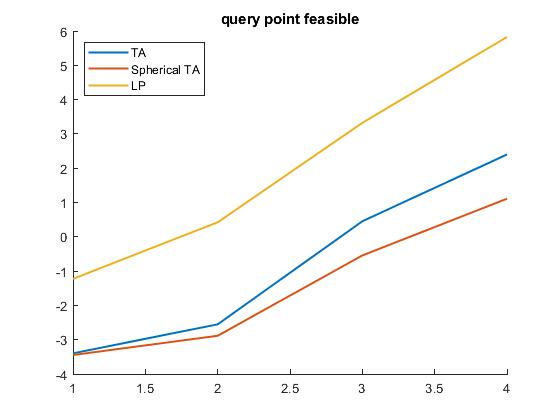
\includegraphics[width=\linewidth]{fea.jpg}
	\end{subfigure}
	\begin{subfigure}[b]{0.45\linewidth}
		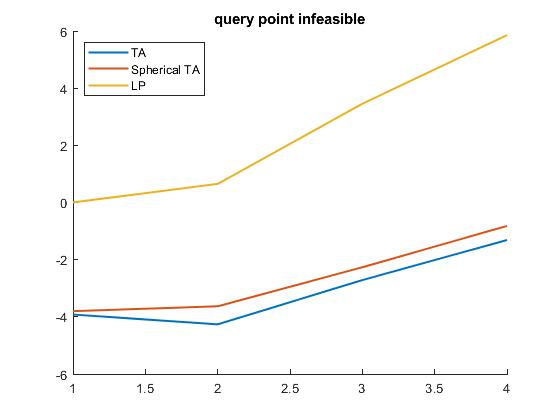
\includegraphics[width=\linewidth]{infea.jpg}
	\end{subfigure}
	\caption{Running time of three algorithms on different size of problems.}
	\label{fig1}
\end{figure}

\newpage
\bibliographystyle{plain}
\bibliography{acmart}
\end{document}
